%ssms

\documentclass[../../main/main.tex]{subfiles}




\begin{document}
\title{Secure State Machine Model}

%%%%%%%%%%%%%%%%%%%%% Chapter SSM Model %%%%%%%%%%%%%%%
\chapter{Secure State Machine Model}\label{chp:ssmmodel}

      %%%%%%%%%%%%%%%%%%% Section State Machines %%%%%%%%%%%%%
\section{State Machines}\label{sec:sm}
State machines are models of systems.  They use \textit{states} and \textit{transitions} among states to describe the system's behavior.  To use the state machine model for a system the system must be describable as states which can change based on some input.    

There are several models of state machines.  A discussion of these models in beyond the scope of this master thesis.  The state machine model described in this master thesis changes states and outputs based on input.  This means that some input will cause the state machine to change states and produce an output.

\subsection{States}
States of a state machine can be nearly anything.  For example, the state for a based could be described by the number of people on base.  If a soldier is permitted to enter the base, then the state of the base increases from n people to n + 1 people. Or, the state of a soldier requesting access to a base could be ``not granted" or ``granted."

In this master thesis, states are phases of the patrol base operations.  For example, figure \ref{pbtoplevel2} shows the top level diagram depicting 6 abstract phases of the patrol base operations.  These abstract phases are the states of the top level state machine.

\begin{figure}[h]
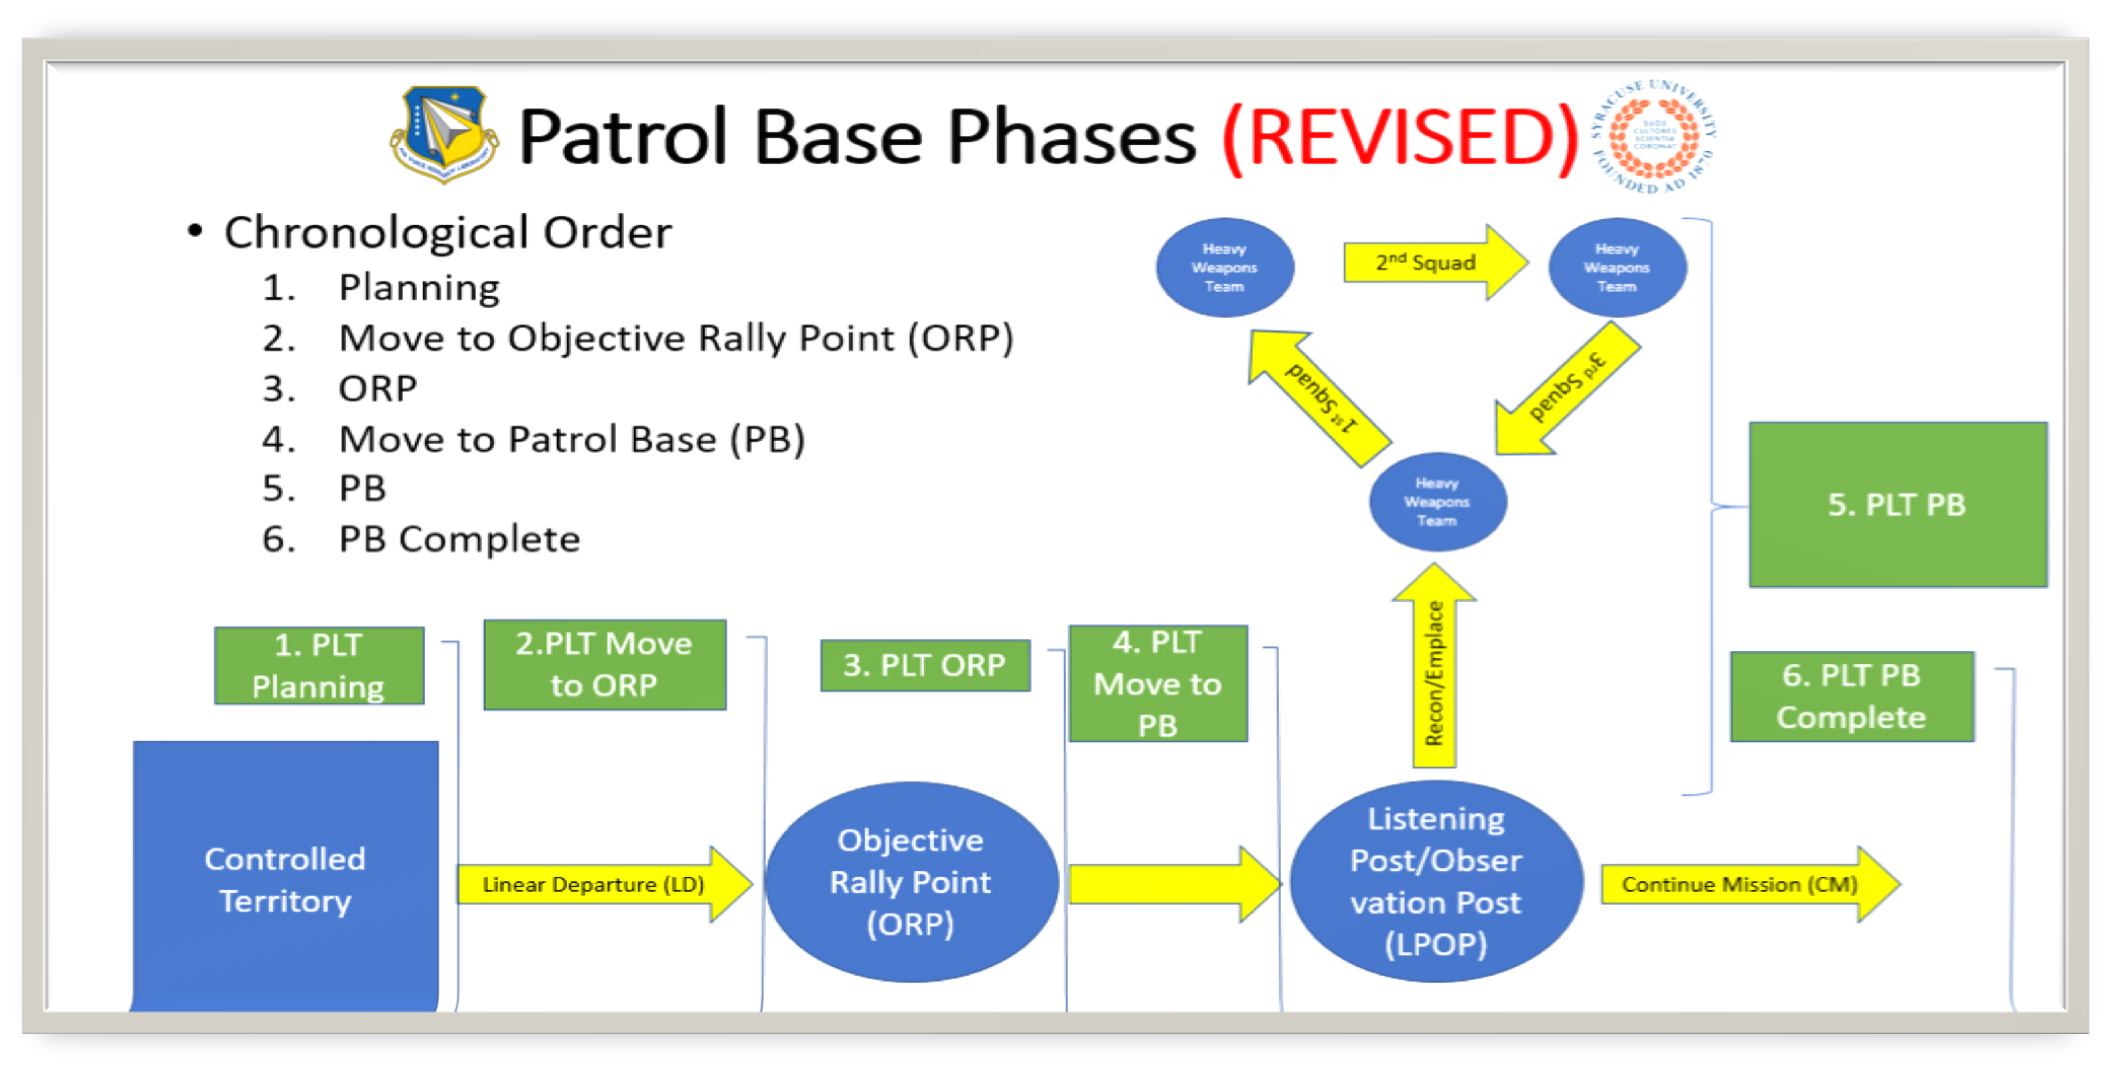
\includegraphics[width=\textwidth]{../figures/pbtoplevel}
\caption{\label{pbtoplevel2}A diagram of the most abstract level in the hierarchy of secure state machines.  Image generated by Jesse Nathaniel as part of the research involved in this master thesis.  Shall I get his permission?}
\end{figure}


\subsection{Transition Commands}
Transition commands are inputs to the state machine.  These inputs determine the next-state (and next-output) of the state machine.  To continue with the examples above, input for the transition from n people to n + 1 people could be ``access granted."  This same input could be used to change a soldier's state from ``not granted" to ``granted."

In this master thesis, commands indicate the next state.  For example, in figure \ref{pbtoplevel2}, transition from the Move to Objective Rally Point (ORP) state to the ORP state is indicated by the command ``conductORP."

\subsection{Next-state Function}
The next-state function describes the next state of the state machine given the current state and input.  The function call is denoted  \[ \text{\textit{NS CURRENT_STATE input }}\]For example, the next-state function to change from the n to n + 1 state would look like this: \[\text{\textit{NS N accessGranted = N + 1}}\].  Similarly, for the soldier: \[\text{\textit{NS NOT_GRANTED accessGranted = GRANTED}}\].

In this master thesis, the next-state function contains the line \[\text{\textit{NS MOVE_TO_ORP conductORP = CONDUCT_ORP}}\]

\subsection{Next-output Function}
The next-output function describes the next output of the state machine given the current state and input.  This function call is denoted  \[\text{\textit{NOut CURRENT_STATE input}}\] For example, the next-output function to change from the n to n + 1 state may look like this: \[\text{\textit{NOut N accessGranted = BasePopulationIncreasedByOne}}\].  Similarly, for the soldier: \[\text{\textit{NOut NOT_GRANTED accessGranted = NowOnBase}}\].

In this master thesis, the next-output function contains the line \[\text{\textit{NS MOVE_TO_ORP conductORP = ConductORP}}\]

\subsection{Configuration}
A configuration describes the status of a state machine using there pieces of information: (1) current state, (2) a list of inputs (input stream), and (3) a list of outputs (output stream). The information in the configuration is sufficient to instruct the state machine's next behavior.

\subsection{Transitions}


      %%%%%%%%%%%%%%%%%%% Section Secure State Machines %%%%%%%%%
\section{Secure State Machines}\label{sec:ssm}
Secure state machines add a level of security to the state machine model.  In particular, the secure state machine implements access control by way of complete mediation.   

\subsection{State Machine Versus Secure State Machine}
State machines define states, inputs, outputs, next-state functions, and next-output functions.  Through these means, the state machine defines it's behavior.  Secure state machines add the additional concept of complete mediation to the state machine model by including checks on authentication and authorization.  These checks are performed by a monitor.

 
\subsection{Monitors}\label{monitors}
It is the duty of the monitor to control the behavior of the \glsentryshort{ssm} with regards to complete mediation.  The monitor is a essentially a guard that checks for the proper authentication and authorization for all \glsentryshort{ssm} transition requests.  In a real world analogy, the monitor is the sentry at the gate who checks IDs and determines who is granted access to the base.  In the \glsentryshort{ssm}, the monitor controls access to state machine transitions in the same manner.

\subsection{Transition Types}
The monitor assigns a transition type to each command (or \glsentryshort{ssm} transition request). This assignment is based on the security policy and the rules for authentication.  There are three transition types: execute (\textit{exec}), trap, (\textit{trap}), and discard (\textit{discard})\footnote{The names are derived from their use in virtual machines.  Commands in virtual machines are either executed, trapped, or discarded.  Each has a different behavior in the machine.}.  

\subsubsection{\textit{exec}}
The \textit{exec} transition type indicates that a command should be executed.  For example, if the Platoon Leader issues the command (request) \textit{crossLD}, then the monitor must first check the authentication and authorization for that request.  If the monitor authenticates the Platoon Leader and authorizes her on that request, then the monitor can justify executing that request.  In the \glsentryshort{ssm} model, this means that the transition from the PLAN_PB state to the MOVE_TO_ORP state (indicated by the command \textit{crossLD}) should be allowed. 
\subsubsection{\textit{trap}}
The \textit{trap} transition type indicates that a command should NOT be executed.  The \textit{trap} transition type indicates that the principal is authenticated, but NOT authorized on that command.  For example, if the Platoon Leader issues the command \textit{initiateMovement}, then the monitor must first check the authentication and authorization of that request.  In this case, the monitor authenticates the Platoon Leader.  But, the monitor does not authorize the Platoon Leader on the command \textit{initiateMovement} because only the Platoon Sergeant is authorized on this command.  In the \glsentryshort{ssm} model, this means that the transition from the WARNO state to the REPORT1 state (partially indicated by \textit{initiateMovement}) should NOT be allowed.  It should be trapped.


\subsubsection{\textit{discard}}
Like the \textit{trap} transition type, the \textit{discard} transition type indicates that the command should NOT be executed.  The \textit{discard} transition type indicates that the principal is neither authenticated nor authorized.  It may also indicate that the command is not of the correct form. For example, if SomeGuy issues \textit{anyCommand}, the monitor must first check the authentication and authorization for that request. If the monitor does not authenticate SomeGuy, then SomeGuy's command is discarded.

It is useful to differentiated between the \textit{trap} and \textit{discard} transition types.  This allows for the behavior of the \glsentryshort{ssm} to handle authenticated but unauthorized and un-authenticated and unauthorized commands differently.  For example, a sentry may choose to deny access to someone who is authenticated but unauthorized.  On the other hand, a sentry may choose to detain an unauthenticated person.

\subsection{Commands}
Commands in the \glsentryshort{ssm} are handled differently than in the state machine.  Principals issue commands (make requests).  The monitor inspects the command (request) for proper authentication and authorization and assigns a transition type to the command (request).  This combination of transition type and command (request) is then passed to the next-state and next-output functions.  These functions define how the \glsentryshort{ssm} responds to each transition type and command (request) pair.  This differs from the state machine in that the state machine only defines next-state and next-output functions for commands.  The state machines is not concerned with authentication and authorization (i.e., access-control).

For example, the \glsentryshort{ssm} for the top level is shown in figure \ref{ssmPBDiagram2} (this is the same as figure \ref{ssmPBDiagram} in section \ref{ssec:toplevel}).  

\begin{figure}[h!]
\centering
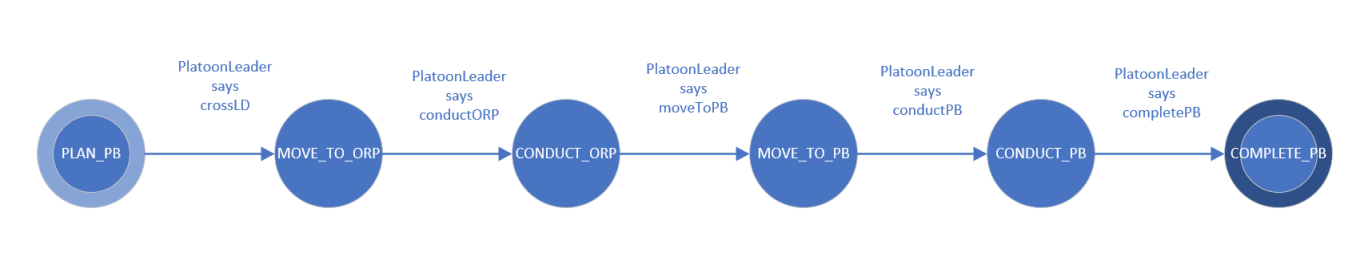
\includegraphics[width=\textwidth]{../figures/ssmPBDiagram}
\caption{\label{ssmPBDiagram2} Top level diagram.}
\end{figure}

In the state machine, the transition from PLAN_PB to MOVE_TO_ORP only requires the command \textit{crossLD}.  But, in the secure state machine, transitions require some form of access-control.  Transitions are indicated by principals making requests of the form \textit{SomePrincipal says someCommand}.  In figure \ref{ssmPBDiagram2}, the Platoon Leader makes a request (issues a command) to transition from the PLAN_PB state to the MOVE_TO_ORP by stating 
 \[\textit{PlatoonLeader says crossLD}.\]

The monitor then checks the authentication and authorization of the principal and returns the command with a transition type.  For example, if the Platoon Leader is both authenticated and authorized on the command \textit{crossLD}, then the monitor returns the transition type and command pair 
\[exec \hspace{0.2cm} crossLD\]

This is passed to the next-state and next-output functions.  The next-state function is then justified in executing the transition from the PLAN_PB state to the MOVE_TO_ORP state.  

\subsection{Authentication}
Authentication in the \glsentryshort{ssm} refers to verification of identity.  Authentication is a very broad topic and details are beyond the scope of this master thesis.  

In this master thesis, authentication is dealt with by simple visual confirmation of a principal's identity\footnote{Although, other methods are discussed in the chapter \ref{chp:other}, particularly with regards to accountability systems.}.  This was justified by assuming that most soldiers in the platoon should recognize their leaders.

Authentication is verified by the monitor on each request\footnote{In the implementation of the \glsentryshort{ssm}, this may or may not be the case.  For example, access to a secured facility may require proper authentication upon entering the facility.  This may be indicated with by a badge worn by the individual while in the facility.  Within the facility, only badges are checked.  But, the process of verifying identity only occurs at the entry.}.  This means that each request must be of the form \textit{SomePrincipal says someCommand}, even if the principal was previously authenticated.  

\subsection{Authorization}
Authentication is a way of controlling who has access to what by means of a security policy.  The security policy implements the principal of complete mediation (and other security policies).  

Authentication in the \glsentryshort{ssm} is typically one or more functions that define which principals have control over which transitions.  A simple authorization in a \glsentryshort{ssm} is \textit{SomePrincipal controls someCommand}.    Using the access-control logic (ACL) described in Chapter \ref{chp:csbdacl} and a request of the form \textit{SomePrincipal says someCommand}, \textit{someCommand} is justified.  Of course, the monitor must first check the authentication of SomePrincipal.  Once that is verified, the monitor returns the transition type and command pair \textit{exec someCommand}.

Authorization is often more complicated.  For example, there are two security policies for the top level \glsentryshort{ssm} shown in figure \ref{ssmPBDiagram2}.  The security policy for the Omni principal is
\[\text{\textit{Omni controls omniCommand}}.\]  This means that the Omni principal is authorized on any omniCommand.  For example, \textit{ssmPlanPBComplete} is one \textit{omniCommand} in the top level \glsentryshort{ssm} in figure \ref{ssmPBDiagram2}.  The security policy for the Platoon Leader depends on the current state because the Platoon Leader is only authorized to transition to the next state if the current state is complete.  (Omni indicates when the current state is complete.)  Thus, the security policy for the Platoon Leader on the transition from the PLAN_PB state to the MOVE_TO_ORP state in figure \ref{ssmPBDiagram2} has the form \[\text{\textit{ssmPlanPBComplete impf PlatoonLeader controls crossLE}}\]where \textit{impf} is the \glsentryshort{acl} operator for implication.

\subsection{Next-state And Next-output Functions}
The next-state and next-output functions define the behavior for the \glsentryshort{ssm}.  Whereas the behavior of the state machine is defined only for states and commands, the behavior in the \glsentryshort{ssm} includes the behavior for each transition type in combination with each command.  This means that for each command, the next-state and next-output functions define three separate behaviors: \textit{exec someCommand}, \textit{trap someCommand}, and \textit{discard someCommand}.  

\subsection{Configurations}
The configuration is a description of the status of the \glsentryshort{ssm} using six pieces of information: (1) an authentication function, (2) a state interpretation function (a state-dependent security policy), (3), a security context, (4) an input list (a command list), (5) a state, and (6) an output list.   The next-state and next-output functions are not part of the configuration because they define the permanent structure of the \glsentryshort{ssm}.


      %%%%%%%%%%%%%%%%%%% Section SSMs in HOL %%%%%%%%%%%%%
\section{Secure State Machines in HOL}\label{sec:sminHOL}

\subsection{Parameterizable Secure State Machine}
\subsection{Input Stream}
The input to the secure state machines is in the form of a list of inputs.  Elements in the list are of the form \textit{P says prop (SOME cmd)}.  It is necessary to extract particular components from the list and list elements.  Several functions are defined to do this.  They are described below.  These are essentially helper functions.

\paragraph*{extractCommand}
extractCommand takes one input of the form \textit{P says prop (SOME cmd)} and extracts the \textit{cmd} part.
\begin{tabbing}
\parskip=8pt
\HOLTokenTurnstile{} \\
\hspace{0.3cm}\HOLConst{extractCommand} (\HOLFreeVar{P} \HOLConst{says} \HOLConst{prop} (\HOLConst{SOME} \HOLFreeVar{cmd})) \HOLSymConst{=} \HOLFreeVar{cmd}
\parskip=18pt
\end{tabbing}

\paragraph*{commandList}
commandList takes an input list consisting of list elements of the form \textit{P says prop (SOME cmd)}.  It returns a list of all the \textit{cmd} elements.
\begin{tabbing}
\parskip=8pt
\HOLTokenTurnstile{} \HOLSymConst{\HOLTokenForall{}}\HOLBoundVar{x}. \\
\hspace{0.3cm} \HOLConst{commandList} \HOLBoundVar{x} \HOLSymConst{=} \HOLConst{MAP} \HOLConst{extractCommand} \HOLBoundVar{x}
\parskip=18pt
\end{tabbing}

\paragraph*{extractPropCommand}
extractPropCommand takes one input of the form \textit{P says prop (SOME cmd)} and extracts the \textit{prop (SOME cmd)} part.
\begin{tabbing}
\parskip=8pt
\HOLTokenTurnstile{}\\
\hspace{0.3cm} \HOLConst{extractPropCommand} (\HOLFreeVar{P} \HOLConst{says} \HOLConst{prop} (\HOLConst{SOME} \HOLFreeVar{cmd})) \HOLSymConst{=} \HOLConst{prop} (\HOLConst{SOME} \HOLFreeVar{cmd})
\parskip=18pt
\end{tabbing}

\paragraph*{propCommand}
propCommand takes an input list consisting of list elements of the form \textit{P says prop (SOME cmd)}.  It returns a list of all the \textit{prop (SOME cmd)} elements.
\begin{tabbing}
\parskip=8pt
\HOLTokenTurnstile{} \HOLSymConst{\HOLTokenForall{}}\HOLBoundVar{x}. \\
\hspace{0.3cm} \HOLConst{propCommandList} \HOLBoundVar{x} \HOLSymConst{=} \HOLConst{MAP} \HOLConst{extractPropCommand} \HOLBoundVar{x}
\parskip=18pt
\end{tabbing}


\paragraph*{extractInput}
extractInput takes one input of the form \textit{P says prop x} and extracts the \textit{x} part. Note that \textit{x} can have two forms: \textit{NONE} or \textit{SOME cmd}.
\begin{tabbing}
\parskip=8pt
\HOLTokenTurnstile{}\\
\hspace{0.3cm} \HOLConst{extractInput} (\HOLFreeVar{P} \HOLConst{says} \HOLConst{prop} \HOLFreeVar{x}) \HOLSymConst{=} \HOLFreeVar{x}
\parskip=18pt
\end{tabbing}

\paragraph*{inputList}
inputList takes an input list consisting of list elements of the form \textit{P says prop x}.  It returns a list of all the \textit{x} elements.
\begin{tabbing}
\parskip=8pt
\HOLTokenTurnstile{} \HOLSymConst{\HOLTokenForall{}}\HOLBoundVar{xs}. \\
\hspace{0.3cm} \HOLConst{inputList} \HOLBoundVar{xs} \HOLSymConst{=} \HOLConst{MAP} \HOLConst{extractInput} \HOLBoundVar{xs}
\parskip=18pt
\end{tabbing}


\subsection{Commands}
\paragraph*{Option Type}
The option type allows for the return of "no value."  In functional programming, this is an important concept because functions must always return a value.  Consider the following example.
Consider a search for the letter associated with the number 1 in an association list of the form \{('a',1), ('b',2), ... (a,26)\}. In this case, the search returns the integer value 'a'.  But, what if the target of the search is the number 27?  The search must return something.  But, there is nothing to return.  This is where the option type comes in handy.  Instead of returning 'a' for 1 and 'b' for 2 and so on, the search returns SOME 'a' and SOME 'b' and so on.  If the search does not find a match, it returns NONE.

The definition for the option datatype is shown below.

\HOLFreeVar{option} = \HOLConst{NONE} \HOLTokenBar{} \HOLConst{SOME} 'a

In the datatype definition above, 'a is replaced with some other datatype.  

\paragraph*{A Closer Look at Commands}
To see how this works, it is necessary to define some other datatypes. The OMNILevel folder in OMNITypesScript.sml contains definitions that are used in all secure state machines. One definition is the \HOLFreeVar{command} datatype definition.

\begin{tabbing}
\HOLFreeVar{command} = \HOLConst{ESCc} \HOLTyOp{escCommand} \HOLTokenBar{} \HOLConst{SLc} 'slCommand
\end{tabbing}

The \HOLFreeVar{command} datatype consists of two additional datatypes: \HOLConst{ESCc} \HOLTyOp{escCommand} and \HOLConst{SLc} 'slCommand.  Note that the first part of each of these are the datatype constructors\footnote{see the background section \ref{sec:adtinml}}: \HOLConst{ESCc} and \HOLConst{SLc}.  The second part is the name of the datatype variable\footnote{Both of these are datatype variables because they define other datatypes.} or datatype.  

The first datatype refers to the escape commands.  They are defined as \HOLTyOp{escCommand} in the same file as \HOLFreeVar{command}.

 \begin{tabbing}
 \HOLFreeVar{escCommand} = \= \HOLConst{returnToBase} \\
 						\>\HOLTokenBar{} \HOLConst{changeMission} \\
						\>\HOLTokenBar{} \HOLConst{resupply}
           \HOLTokenBar{} \HOLConst{reactToContact}
\end{tabbing}

This datatype definition defines three commands (or datatype values) which represent escape conditions in the patrol base operations.  

The second dataytpe variable 'slCommand refers to the state-level commands.  These are defined further in each secure state machine.  

Notice that there is a tick mark (apostrophe) before 'slCommand and not before \HOLTyOp{escCommand}.  In general, the tick mark in \glsentryshort{hol} represents an undefined dataytpe.  In this case, 'slCommand is not yet defined (because it is defined elsewhere), whereas the definition for \HOLTyOp{escCommand} is defined in the same file and above the definition for \HOLFreeVar{command}.   

An example of a definition for 'slCommand can be found in the top level \glsentryshort{ssm}.  It is defined in the folder topLevel and in the file PBIntegratedTypeScript.sml file.

\HOLFreeVar{slCommand} = \HOLConst{PL} \HOLTyOp{plCommand} \HOLTokenBar{} \HOLConst{OMNI} \HOLTyOp{omniCommand}

This is defined similarly to \HOLFreeVar{command}.  There are two datatypes that make-up the datatype \HOLFreeVar{slCommand}.  None of these have tick marks, which means both of these are defined.  In particular, they are both defined in the same file as \HOLFreeVar{slCommand}.

\HOLFreeVar{plCommand} refers to the Platoon Leader commands.  These are commands that the Platoon Leader is authorized to make.  

\begin{tabbing}
\HOLFreeVar{plCommand} = \= \HOLConst{crossLD} \\
					     \>\HOLTokenBar{} \HOLConst{conductORP} \\
					     \>\HOLTokenBar{} \HOLConst{moveToPB} \\
					     \>\HOLTokenBar{} \HOLConst{conductPB}\\
         				     \> \HOLTokenBar{} \HOLConst{completePB} \\
				             \> \HOLTokenBar{} \HOLConst{incomplete}
\end{tabbing}


\HOLFreeVar{omniCommand} refers to commands that the OMNI level principal\footnote{See section \ref{ssec:omnilevel} for a discussion of the OMNI level principal.} is authorized to make. 

\begin{tabbing}
\HOLFreeVar{omniCommand} = \= \HOLConst{ssmPlanPBComplete} \\
						 \> \HOLTokenBar{} \HOLConst{ssmMoveToORPComplete}\\
 				       	 	 \> \HOLTokenBar{} \HOLConst{ssmConductORPComplete} \\
						 \> \HOLTokenBar{} \HOLConst{ssmMoveToPBComplete}\\
            					 \> \HOLTokenBar{} \HOLConst{ssmConductPBComplete}\\
					 	 \> \HOLTokenBar{} \HOLConst{invalidOmniCommand}
\end{tabbing}          
          
          
\paragraph*{Option Type with Commands}
With these definitions, it is possible to see how the options types are used with commands (datatypes).  What follows is a list of examples using the option types and commands (datatypes) described above.  The type signatures are also included because it will help the reader recognize them in the \glsentryshort{hol} code.
\begin{description}
\item[ ] SOME (SLc (ESCc returnToBase)) \\
The type for this is escCommand Option
The type for this is (escCommand command)Option.
\item[ ] SOME (SLc (PL moveToORP))  \\
The type for this is ((plCommand slCommand) command)Option.  
\item[ ] SOME (SLc (OMNI ssmMoveToORPComplete))\\
The type for this is ((omniCommand slCommand) command)Option.  
\end{description}

Note that the constructors are necessary for each command. Also, note that in the \glsentryshort{hol} code for the patrol base operations, the reader will typically see (slCommand command)Option.  This is because the definitions require a type \HOLFreeVar{slCommand}, which includes \HOLFreeVar{plCommand}  and \HOLFreeVar{omniCommand}.




\subsubsection{Transition Types}
Transition datatypes indicate how a command is handled by the monitor.  The three transition datatypes are described below. 

\HOLFreeVar{trType} = \HOLConst{discard} 'cmdlist \HOLTokenBar{} \HOLConst{trap} 'cmdlist \HOLTokenBar{} \HOLConst{exec} 'cmdlist

The 'cmdlist refers to a list of commands of the form discussed in the section above.  For example, to execute the transition from the PLAN_PB state to the MOVE_TO_ORP state, the monitor must return the transition type and command pair with the later of the pair in the form of a list 
\[\text{\textit{exec [SOME (SLc (PL crossLD))]}} \]

where \textit{SOME (SLc (PL crossLD))} is the single item in the cmdlist.  The transition type with the command list is then passed to the next-state and next-output functions.

\subsection{Authentication}
Authorization is context dependent. But, a parametrizable authentication is defined in the parametrizable \glsentryshort{ssm}.

\begin{tabbing}
\parskip=8pt

\HOLTokenTurnstile{} \=\HOLSymConst{\HOLTokenForall{}}\HOLBoundVar{elementTest} \HOLBoundVar{x}. \\
    \> \HOLConst{authenticationTest} \HOLBoundVar{elementTest} \HOLBoundVar{x}  \HOLSymConst{\HOLTokenEquiv{}} \\
    \> \HOLConst{FOLDR} (\HOLTokenLambda{}\HOLBoundVar{p} \HOLBoundVar{q}. \HOLBoundVar{p} \HOLSymConst{\HOLTokenConj{}} \HOLBoundVar{q}) \HOLConst{T} (\HOLConst{MAP} \HOLBoundVar{elementTest} \HOLBoundVar{x})
\parskip=18pt
\end{tabbing}

This function takes an elementTest function and an input list as parameters.  The elementTest function is named inputOK and it is defined separately for each \glsentryshort{ssm}.  elementTest takes a single input of the form \textit{SomePrincipal says someCommand}.  It returns TT (the \glsentryshort{acl} representation of True) if the input is authenticated and FF otherwise.  The authenticationTest function FOLDRs the elementTest function over the input list x with the conjunction function and True as the accumulator\footnote{This means that the elementTest function is applied to each element in the input list x, resulting in a TT or FF value for each element in the input list x.   Then, in essence, the value of the conjunction of all these values is returned.}  Thus, if all the input elements in the input list x pass the elementTest, the authenticationTest function returns true, otherwise it returns false.  
     
\subsection{Authorization}
Authorization is the security context and it is \glsentryshort{ssm}-dependent. This means that each \glsentryshort{ssm} defines its own security context.  The parametrizable \glsentryshort{ssm} allows for two ways to define the security context and pass them as parameters.  The first is the state interpretation function. This function takes a state and an input list as parameters.  It defines the security context based on state.  All state-dependent behavior may also be defined in this function.

The second function is the security context function.  It takes only the input list as a parameter.  It defines the security context based that is true for any state.

\subsection{Next-state And Next-output Functions}
The next-state and next-output functions are parameters to the parametrizable \glsentryshort{ssm}.  They are defined separately in each \glsentryshort{ssm}.  In the parametrizable \glsentryshort{ssm} they are denoted by NS and Out, respectively.

\subsection{Configurations}
Configurations in the \glsentryshortpl{ssm} have six components.  Each components are defined separately in the \glsentryshortpl{ssm}.  The \glsentryshortpl{ssm} must define each of the six components to use the parametrizable \glsentryshort{ssm}.  These components are:
\begin{enumerate}
\item authentication test function.  \\
The type signature is 

\hspace{0.5cm}  (('command \HOLTyOp{option}, 'principal, 'd, 'e) \HOLTyOp{Form} -> \HOLTyOp{bool})

\item state interpretation function.  \\
The type signature is
\begin{tabbing}
\hspace{0.5cm}('state -> \=('command \HOLTyOp{option}, 'principal, 'd, 'e) \HOLTyOp{Form} \HOLTyOp{list} -> \\
				      \>('command \HOLTyOp{option}, 'principal, 'd, 'e) \HOLTyOp{Form} \HOLTyOp{list}) 
\end{tabbing}
\item security context function.  \\
The type signature is 

 \hspace{0.5cm}   (('command \HOLTyOp{option}, 'principal, 'd, 'e) \HOLTyOp{Form} \HOLTyOp{list} -> \\
\hspace{0.5cm}    ('command \HOLTyOp{option}, 'principal, 'd, 'e) \HOLTyOp{Form} \HOLTyOp{list}) 

\item input list stream.  \\
The type signature is

 \hspace{0.5cm}  (('command \HOLTyOp{option}, 'principal, 'd, 'e) \HOLTyOp{Form} \HOLTyOp{list} \HOLTyOp{list}) \

\item state.  \\
The type signature is

\hspace{0.5cm}   'state

\item output stream.  \\
The type signature is 

\hspace{0.5cm} ('output \HOLTyOp{list})
\end{enumerate}

The definition for the configuration datatype is shown below.

\begin{tabbing}
\parskip=8pt
\HOLFreeVar{configuration} = \\
\hspace{0.3cm}    \HOLConst{CFG} \\
\hspace{0.5cm}  (('command \HOLTyOp{option}, 'principal, 'd, 'e) \HOLTyOp{Form} -> \HOLTyOp{bool})\\
\hspace{0.5cm}    ('state -> ('command \HOLTyOp{option}, 'principal, 'd, 'e) \HOLTyOp{Form} \HOLTyOp{list} -> \\
\hspace{0.5cm}    ('command \HOLTyOp{option}, 'principal, 'd, 'e) \HOLTyOp{Form} \HOLTyOp{list}) \\
 \hspace{0.5cm}   (('command \HOLTyOp{option}, 'principal, 'd, 'e) \HOLTyOp{Form} \HOLTyOp{list} -> \\
\hspace{0.5cm}    ('command \HOLTyOp{option}, 'principal, 'd, 'e) \HOLTyOp{Form} \HOLTyOp{list}) \\
 \hspace{0.5cm}  (('command \HOLTyOp{option}, 'principal, 'd, 'e) \HOLTyOp{Form} \HOLTyOp{list} \HOLTyOp{list}) \\
\hspace{0.5cm}   'state \\
\hspace{0.5cm} ('output \HOLTyOp{list})
\parskip=18pt
\end{tabbing}

CFG is the constructor for the datatype.

\subsection{Configuration Interpretation}
The monitor must interpret the configuration.  The CFGInterpret function take as input a Kripke structure and a configuration.  It returns a conjunction of three things: a satList of the security context, a satList of the input stream, and a satList of the stateInterpretation function.  

satList is a list of elements that satisfy the property of soundness as discussed in chapter \ref{chp:csbdacl} section \ref{sssec:soundness}\footnote{Note that in the \glsentryshort{acl} implementation of the "satisfies" and "soundness" properties, "satisfies" serves as "soundness" when it is generalized for all Kripke structures.}.  satList is defined in satListTheory.  

\begin{tabbing}
\parskip=8pt
\HOLTokenTurnstile{} \hspace{0.3cm}\HOLSymConst{\HOLTokenForall{}}\HOLBoundVar{M} \HOLBoundVar{Oi} \HOLBoundVar{Os} \HOLBoundVar{formList}.\\
\hspace{0.5cm}(\HOLBoundVar{M}\HOLSymConst{,}\HOLBoundVar{Oi}\HOLSymConst{,}\HOLBoundVar{Os}) \HOLConst{satList} \HOLBoundVar{formList} \HOLSymConst{\HOLTokenEquiv{}} \\
\hspace{0.5cm} \HOLConst{FOLDR} (\HOLTokenLambda{}\HOLBoundVar{x} \HOLBoundVar{y}. \HOLBoundVar{x} \HOLSymConst{\HOLTokenConj{}} \HOLBoundVar{y}) \HOLConst{T} (\HOLConst{MAP} (\HOLTokenLambda{}\HOLBoundVar{f}. (\HOLBoundVar{M}\HOLSymConst{,}\HOLBoundVar{Oi}\HOLSymConst{,}\HOLBoundVar{Os}) \HOLConst{sat} \HOLBoundVar{f}) \HOLBoundVar{formList})
\parskip=18pt
\end{tabbing}

satList MAPs the \textit{sat} operator onto each element in the formList. It then FOLDRs the formList elements with the conjunction function and accumulator True.  This means that satList applied to formList returns true if each element in the list satisfies the \textit{sat} property.

Other properties of satList can be found in appendix \ref{ppacl}.

With satList defined, the meaning of CFGInterpret should follow.  

\begin{tabbing}
\parskip=8pt
\HOLTokenTurnstile{} \HOLConst{CFGInterpret}\\
\hspace{0.5cm}(\HOLFreeVar{M}\HOLSymConst{,}\HOLFreeVar{Oi}\HOLSymConst{,}\HOLFreeVar{Os})
     (\HOLConst{CFG} \HOLFreeVar{elementTest} \HOLFreeVar{stateInterp} \HOLFreeVar{context} (\HOLFreeVar{x}\HOLSymConst{::}\HOLFreeVar{ins}) \HOLFreeVar{state}
     \HOLFreeVar{outStream}) \HOLSymConst{\HOLTokenEquiv{}} \\
\hspace{0.5cm}(\HOLFreeVar{M}\HOLSymConst{,}\HOLFreeVar{Oi}\HOLSymConst{,}\HOLFreeVar{Os}) \HOLConst{satList} \HOLFreeVar{context} \HOLFreeVar{x} \HOLSymConst{\HOLTokenConj{}} (\HOLFreeVar{M}\HOLSymConst{,}\HOLFreeVar{Oi}\HOLSymConst{,}\HOLFreeVar{Os}) \HOLConst{satList} \HOLFreeVar{x} \HOLSymConst{\HOLTokenConj{}}\\
\hspace{0.5cm}(\HOLFreeVar{M}\HOLSymConst{,}\HOLFreeVar{Oi}\HOLSymConst{,}\HOLFreeVar{Os}) \HOLConst{satList} \HOLFreeVar{stateInterp} \HOLFreeVar{state} \HOLFreeVar{x}
\parskip=18pt
\end{tabbing}

\subsection{Transition Definitions}
Transitions are defined in \glsentryshort{hol} 
\paragraph*{rule0}
\parskip=8pt
\begin{tabbing}
\HOLTokenTurnstile{} \\
\hspace{0.3cm}\HOLConst{TR} (\HOLFreeVar{M}\HOLSymConst{,}\HOLFreeVar{Oi}\HOLSymConst{,}\HOLFreeVar{Os}) (\HOLConst{exec} (\HOLConst{inputList} \HOLFreeVar{x}))\\
\hspace{0.5cm}(\HOLConst{CFG} \\
\hspace{0.9cm}\HOLFreeVar{elementTest} \\
\hspace{0.9cm}\HOLFreeVar{stateInterp} \\
\hspace{0.9cm}\HOLFreeVar{context} \\
\hspace{0.9cm}(\HOLFreeVar{x}\HOLSymConst{::}\HOLFreeVar{ins}) \\
\hspace{0.9cm}\HOLFreeVar{s} \\
\hspace{0.9cm}\HOLFreeVar{outs})\\
\hspace{0.5cm}(\HOLConst{CFG} \\
\hspace{0.9cm}\HOLFreeVar{elementTest} \\
\hspace{0.9cm}\HOLFreeVar{stateInterp} \\
\hspace{0.9cm}\HOLFreeVar{context} \\
\hspace{0.9cm}\HOLFreeVar{ins}\\
\hspace{0.9cm}(\HOLFreeVar{NS} \HOLFreeVar{s} (\HOLConst{exec} (\HOLConst{inputList} \HOLFreeVar{x})))\\
\hspace{0.9cm}(\HOLFreeVar{Out} \HOLFreeVar{s} (\HOLConst{exec} (\HOLConst{inputList} \HOLFreeVar{x}))\HOLSymConst{::}\HOLFreeVar{outs})) \\
\hspace{0.3cm}\HOLSymConst{\HOLTokenEquiv{}}\HOLConst{authenticationTest} \HOLFreeVar{elementTest} \HOLFreeVar{x} \\
\hspace{0.3cm}\HOLSymConst{\HOLTokenConj{}}\HOLConst{CFGInterpret} (\HOLFreeVar{M}\HOLSymConst{,}\HOLFreeVar{Oi}\HOLSymConst{,}\HOLFreeVar{Os})\\
\hspace{0.5cm}(\HOLConst{CFG} \\
\hspace{0.9cm}\HOLFreeVar{elementTest} \\
\hspace{0.9cm}\HOLFreeVar{stateInterp} \\
\hspace{0.9cm}\HOLFreeVar{context} \\
\hspace{0.9cm}(\HOLFreeVar{x}\HOLSymConst{::}\HOLFreeVar{ins}) \\
\hspace{0.9cm}\HOLFreeVar{s} \\
\hspace{0.9cm}\HOLFreeVar{outs})
\end{tabbing}
\parskip=18pt


\paragraph*{rule1}
\begin{tabbing}
\parskip=8pt
\HOLTokenTurnstile{} \\
\hspace{0.3cm}\HOLConst{TR} (\HOLFreeVar{M}\HOLSymConst{,}\HOLFreeVar{Oi}\HOLSymConst{,}\HOLFreeVar{Os}) (\HOLConst{trap} (\HOLConst{inputList} \HOLFreeVar{x}))\\
\hspace{0.5cm}(\HOLConst{CFG} \\
\hspace{0.9cm}\HOLFreeVar{elementTest} \\
\hspace{0.9cm}\HOLFreeVar{stateInterp} \\
\hspace{0.9cm}\HOLFreeVar{context} \\
\hspace{0.9cm}(\HOLFreeVar{x}\HOLSymConst{::}\HOLFreeVar{ins}) \\
\hspace{0.9cm}\HOLFreeVar{s} \\
\hspace{0.9cm}\HOLFreeVar{outs})\\
\hspace{0.5cm}(\HOLConst{CFG} \\
\hspace{0.9cm}\HOLFreeVar{elementTest} \\
\hspace{0.9cm}\HOLFreeVar{stateInterp} \\
\hspace{0.9cm}\HOLFreeVar{context} \\
\hspace{0.9cm}\HOLFreeVar{ins}\\
\hspace{0.9cm}(\HOLFreeVar{NS} \HOLFreeVar{s} (\HOLConst{trap} (\HOLConst{inputList} \HOLFreeVar{x})))\\
\hspace{0.9cm}(\HOLFreeVar{Out} \HOLFreeVar{s} (\HOLConst{trap} (\HOLConst{inputList} \HOLFreeVar{x}))\HOLSymConst{::}\HOLFreeVar{outs})) \\
\hspace{0.3cm}\HOLSymConst{\HOLTokenEquiv{}} \HOLConst{authenticationTest} \HOLFreeVar{elementTest} \HOLFreeVar{x} \\
\hspace{0.3cm}\HOLSymConst{\HOLTokenConj{}} \HOLConst{CFGInterpret} (\HOLFreeVar{M}\HOLSymConst{,}\HOLFreeVar{Oi}\HOLSymConst{,}\HOLFreeVar{Os})\\
\hspace{0.5cm}(\HOLConst{CFG} \\
\hspace{0.9cm}\HOLFreeVar{elementTest} \\
\hspace{0.9cm}\HOLFreeVar{stateInterp} \\
\hspace{0.9cm}\HOLFreeVar{context} \\
\hspace{0.9cm}(\HOLFreeVar{x}\HOLSymConst{::}\HOLFreeVar{ins}) \\
\hspace{0.9cm}\HOLFreeVar{s} \\
\hspace{0.9cm}\HOLFreeVar{outs})
\parskip=18pt
\end{tabbing}

\paragraph*{rule2}
\begin{tabbing}
\parskip=8pt
\HOLTokenTurnstile{} \\
\hspace{0.3cm}(\HOLConst{TR} (\HOLFreeVar{M}\HOLSymConst{,}\HOLFreeVar{Oi}\HOLSymConst{,}\HOLFreeVar{Os}) (\HOLConst{discard} (\HOLConst{inputList} \HOLFreeVar{x}))\\
\hspace{0.5cm}(\HOLConst{CFG} \\
\hspace{0.9cm}\HOLFreeVar{elementTest} \\
\hspace{0.9cm}\HOLFreeVar{stateInterp} \\
\hspace{0.9cm}\HOLFreeVar{context} \\
\hspace{0.9cm}(\HOLFreeVar{x}\HOLSymConst{::}\HOLFreeVar{ins}) \\
\hspace{0.9cm}\HOLFreeVar{s} \HOLFreeVar{outs})\\
\hspace{0.5cm}(\HOLConst{CFG} \\
\hspace{0.9cm}\HOLFreeVar{elementTest}\\
\hspace{0.9cm}\HOLFreeVar{stateInterp} \\
\hspace{0.9cm}\HOLFreeVar{context} \\
\hspace{0.9cm}\HOLFreeVar{ins}\\
\hspace{0.9cm}(\HOLFreeVar{NS} \HOLFreeVar{s} (\HOLConst{discard} (\HOLConst{inputList} \HOLFreeVar{x})))\\
\hspace{0.9cm}(\HOLFreeVar{Out} \HOLFreeVar{s} (\HOLConst{discard} (\HOLConst{inputList} \HOLFreeVar{x}))\HOLSymConst{::}\HOLFreeVar{outs})) \\
\hspace{0.3cm}\HOLSymConst{\HOLTokenEquiv{}}\\
\hspace{0.3cm}\HOLSymConst{\HOLTokenNeg{}}\HOLConst{authenticationTest} \HOLFreeVar{elementTest} \HOLFreeVar{x})
\parskip=18pt
\end{tabbing}


\paragraph*{TR_exec_cmd_rule}
\begin{tabbing}
\parskip=8pt
\HOLTokenTurnstile{} \\
\hspace{0.3cm}\HOLSymConst{\HOLTokenForall{}}\HOLBoundVar{elementTest} \HOLBoundVar{context} \HOLBoundVar{stateInterp} \HOLBoundVar{x} \HOLBoundVar{ins} \HOLBoundVar{s} \HOLBoundVar{outs}.\\
\hspace{0.5cm}(\HOLSymConst{\HOLTokenForall{}}\HOLBoundVar{M} \HOLBoundVar{Oi} \HOLBoundVar{Os}.\\
\hspace{0.9cm}\HOLConst{CFGInterpret} (\HOLBoundVar{M}\HOLSymConst{,}\HOLBoundVar{Oi}\HOLSymConst{,}\HOLBoundVar{Os})\\
\hspace{1.1cm}(\HOLConst{CFG} \\
\hspace{1.3cm}\HOLBoundVar{elementTest} \\
\hspace{1.3cm}\HOLBoundVar{stateInterp} \\
\hspace{1.3cm}\HOLBoundVar{context} \\
\hspace{1.3cm}(\HOLBoundVar{x}\HOLSymConst{::}\HOLBoundVar{ins}) \\
\hspace{1.3cm}\HOLBoundVar{s}\\
\hspace{1.3cm}\HOLBoundVar{outs}) \\
\hspace{0.9cm}\HOLSymConst{\HOLTokenImp{}}(\HOLBoundVar{M}\HOLSymConst{,}\HOLBoundVar{Oi}\HOLSymConst{,}\HOLBoundVar{Os}) \HOLConst{satList} \HOLConst{propCommandList} \HOLBoundVar{x}) \\
\hspace{0.5cm}\HOLSymConst{\HOLTokenImp{}} \HOLSymConst{\HOLTokenForall{}}\HOLBoundVar{NS} \HOLBoundVar{Out} \HOLBoundVar{M} \HOLBoundVar{Oi} \HOLBoundVar{Os}.\\
\hspace{0.9cm}\HOLConst{TR} (\HOLBoundVar{M}\HOLSymConst{,}\HOLBoundVar{Oi}\HOLSymConst{,}\HOLBoundVar{Os}) (\HOLConst{exec} (\HOLConst{inputList} \HOLBoundVar{x}))\\
\hspace{1.1cm}(\HOLConst{CFG} \\
\hspace{1.3cm}\HOLBoundVar{elementTest} \\
\hspace{1.3cm}\HOLBoundVar{stateInterp} \\
\hspace{1.3cm}\HOLBoundVar{context} \\
\hspace{1.3cm}(\HOLBoundVar{x}\HOLSymConst{::}\HOLBoundVar{ins}) \\
\hspace{1.3cm}\HOLBoundVar{s} \\
\hspace{1.3cm}\HOLBoundVar{outs})\\
\hspace{1.1cm}(\HOLConst{CFG} \\
\hspace{1.3cm}\HOLBoundVar{elementTest} \\
\hspace{1.3cm}\HOLBoundVar{stateInterp} \\
\hspace{1.3cm}\HOLBoundVar{context} \\
\hspace{1.3cm}\HOLBoundVar{ins}\\
\hspace{1.3cm}(\HOLBoundVar{NS} \HOLBoundVar{s} (\HOLConst{exec} (\HOLConst{inputList} \HOLBoundVar{x})))\\
\hspace{1.3cm}(\HOLBoundVar{Out} \HOLBoundVar{s} (\HOLConst{exec} (\HOLConst{inputList} \HOLBoundVar{x}))\HOLSymConst{::}\HOLBoundVar{outs})) \\
\hspace{0.5cm}\HOLSymConst{\HOLTokenEquiv{}} \HOLConst{authenticationTest} \HOLBoundVar{elementTest} \HOLBoundVar{x} \\
\hspace{0.5cm}\HOLSymConst{\HOLTokenConj{}} \HOLConst{CFGInterpret} (\HOLBoundVar{M}\HOLSymConst{,}\HOLBoundVar{Oi}\HOLSymConst{,}\HOLBoundVar{Os})\\
\hspace{0.9cm}(\HOLConst{CFG} \\
\hspace{1.1cm}\HOLBoundVar{elementTest} \\
\hspace{1.1cm}\HOLBoundVar{stateInterp} \\
\hspace{1.1cm}\HOLBoundVar{context} \\
\hspace{1.1cm}(\HOLBoundVar{x}\HOLSymConst{::}\HOLBoundVar{ins}) \\
\hspace{1.1cm}\HOLBoundVar{s} \\
\hspace{1.1cm}\HOLBoundVar{outs}) \\
\hspace{0.5cm}\HOLSymConst{\HOLTokenConj{}} (\HOLBoundVar{M}\HOLSymConst{,}\HOLBoundVar{Oi}\HOLSymConst{,}\HOLBoundVar{Os}) \HOLConst{satList} \HOLConst{propCommandList} \HOLBoundVar{x}
\parskip=18pt
\end{tabbing}

\paragraph*{TR_trap_cmd_rule}
\begin{tabbing}
\parskip=8pt
\HOLTokenTurnstile{} \\
\hspace{0.3cm}\HOLSymConst{\HOLTokenForall{}}\HOLBoundVar{elementTest} \HOLBoundVar{context} \HOLBoundVar{stateInterp} \HOLBoundVar{x} \HOLBoundVar{ins} \HOLBoundVar{s} \HOLBoundVar{outs}.\\
\hspace{0.5cm} (\HOLSymConst{\HOLTokenForall{}}\HOLBoundVar{M} \HOLBoundVar{Oi} \HOLBoundVar{Os}.\\
\hspace{0.9cm}\HOLConst{CFGInterpret} (\HOLBoundVar{M}\HOLSymConst{,}\HOLBoundVar{Oi}\HOLSymConst{,}\HOLBoundVar{Os})\\
\hspace{1.1cm}(\HOLConst{CFG} \\
\hspace{1.3cm}\HOLBoundVar{elementTest} \\
\hspace{1.3cm}\HOLBoundVar{stateInterp} \\
\hspace{1.3cm}\HOLBoundVar{context} \\
\hspace{1.3cm}(\HOLBoundVar{x}\HOLSymConst{::}\HOLBoundVar{ins}) \\
\hspace{1.3cm}\HOLBoundVar{s}\\
\hspace{1.3cm}\HOLBoundVar{outs}) \\
\hspace{0.9cm}\HOLSymConst{\HOLTokenImp{}} (\HOLBoundVar{M}\HOLSymConst{,}\HOLBoundVar{Oi}\HOLSymConst{,}\HOLBoundVar{Os}) \HOLConst{sat} \HOLConst{prop} \HOLConst{NONE}) \\
\hspace{0.5cm}\HOLSymConst{\HOLTokenImp{}} \HOLSymConst{\HOLTokenForall{}}\HOLBoundVar{NS} \HOLBoundVar{Out} \HOLBoundVar{M} \HOLBoundVar{Oi} \HOLBoundVar{Os}.\\
\hspace{0.9cm}\HOLConst{TR} (\HOLBoundVar{M}\HOLSymConst{,}\HOLBoundVar{Oi}\HOLSymConst{,}\HOLBoundVar{Os}) (\HOLConst{trap} (\HOLConst{inputList} \HOLBoundVar{x}))\\
\hspace{1.1cm}(\HOLConst{CFG} \\
\hspace{1.3cm}\HOLBoundVar{elementTest} \\
\hspace{1.3cm}\HOLBoundVar{stateInterp} \\
\hspace{1.3cm}\HOLBoundVar{context} \\
\hspace{1.3cm}(\HOLBoundVar{x}\HOLSymConst{::}\HOLBoundVar{ins}) \\
\hspace{1.3cm}\HOLBoundVar{s} \\
\hspace{1.3cm}\HOLBoundVar{outs})\\
\hspace{1.1cm}(\HOLConst{CFG} \\
\hspace{1.3cm}\HOLBoundVar{elementTest} \\
\hspace{1.3cm}\HOLBoundVar{stateInterp} \\
\hspace{1.3cm}\HOLBoundVar{context} \\
\hspace{1.3cm}\HOLBoundVar{ins}\\
\hspace{1.3cm}(\HOLBoundVar{NS} \HOLBoundVar{s} (\HOLConst{trap} (\HOLConst{inputList} \HOLBoundVar{x})))\\
\hspace{1.3cm}(\HOLBoundVar{Out} \HOLBoundVar{s} (\HOLConst{trap} (\HOLConst{inputList} \HOLBoundVar{x}))\HOLSymConst{::}\HOLBoundVar{outs})) \\
\hspace{0.5cm}\HOLSymConst{\HOLTokenEquiv{}} \HOLConst{authenticationTest} \HOLBoundVar{elementTest} \HOLBoundVar{x} \\
\hspace{0.5cm}\HOLSymConst{\HOLTokenConj{}} \HOLConst{CFGInterpret} (\HOLBoundVar{M}\HOLSymConst{,}\HOLBoundVar{Oi}\HOLSymConst{,}\HOLBoundVar{Os})\\
\hspace{0.9cm}(\HOLConst{CFG} \\
\hspace{1.1cm}\HOLBoundVar{elementTest} \\
\hspace{1.1cm}\HOLBoundVar{stateInterp} \\
\hspace{1.1cm}\HOLBoundVar{context} \\
\hspace{1.1cm}(\HOLBoundVar{x}\HOLSymConst{::}\HOLBoundVar{ins}) \\
\hspace{1.1cm}\HOLBoundVar{s} \\
\hspace{1.1cm}\HOLBoundVar{outs}) \\
\hspace{1.1cm}\HOLSymConst{\HOLTokenConj{}}\\
\hspace{0.5cm}(\HOLBoundVar{M}\HOLSymConst{,}\HOLBoundVar{Oi}\HOLSymConst{,}\HOLBoundVar{Os}) \HOLConst{sat} \HOLConst{prop} \HOLConst{NONE}
\parskip=18pt
\end{tabbing}


\paragraph*{TR_discard_cmd_rule}
\begin{tabbing}
\parskip=8pt
\HOLTokenTurnstile{}\\
\hspace{0.3cm}\HOLConst{TR} (\HOLFreeVar{M}\HOLSymConst{,}\HOLFreeVar{Oi}\HOLSymConst{,}\HOLFreeVar{Os}) (\HOLConst{discard} (\HOLConst{inputList} \HOLFreeVar{x}))\\
\hspace{0.5cm}(\HOLConst{CFG}\\
\hspace{0.9cm}\HOLFreeVar{elementTest}\\ 
\hspace{0.9cm}\HOLFreeVar{stateInterp}\\
\hspace{0.9cm}\HOLFreeVar{context}\\ 
\hspace{0.9cm}(\HOLFreeVar{x}\HOLSymConst{::}\HOLFreeVar{ins})\\
\hspace{0.9cm} \HOLFreeVar{s}\\ 
\hspace{0.9cm}\HOLFreeVar{outs})\\
\hspace{0.5cm}(\HOLConst{CFG}\\ 
\hspace{0.9cm}\HOLFreeVar{elementTest} \\
\hspace{0.9cm}\HOLFreeVar{stateInterp} \\
\hspace{0.9cm}\HOLFreeVar{context} \\
\hspace{0.9cm}\HOLFreeVar{ins}\\
\hspace{0.9cm}(\HOLFreeVar{NS} \HOLFreeVar{s} (\HOLConst{discard} (\HOLConst{inputList} \HOLFreeVar{x})))\\
\hspace{0.9cm}(\HOLFreeVar{Out} \HOLFreeVar{s} (\HOLConst{discard} (\HOLConst{inputList} \HOLFreeVar{x}))\HOLSymConst{::}\HOLFreeVar{outs})) \\
\hspace{0.3cm}\HOLSymConst{\HOLTokenEquiv{}}
   \HOLSymConst{\HOLTokenNeg{}}\HOLConst{authenticationTest} \HOLFreeVar{elementTest} \HOLFreeVar{x}
\parskip=18pt
\end{tabbing}




\end{document}